
% ===========================================================================
% Title:
% ---------------------------------------------------------------------------
% to create Type I fonts type "dvips -P cmz -t letter <filename>"
% ===========================================================================
\documentclass[11pt]{article}       %--- LATEX 2e base
\usepackage{latexsym}               %--- LATEX 2e base
%---------------- Wide format -----------------------------------------------
\textwidth=6in \textheight=9in \oddsidemargin=0.25in
\evensidemargin=0.25in \topmargin=-0.5in
%--------------- Algorithm --------------------------------------------------
\newtheorem{algX}{Algorithm}
\newenvironment{algorithm}       {\begin{algX}\begin{em}}%
                                 {\par\noindent --- End of Algorithm ---
                                 \end{em}\end{algX}}
\newcommand{\step}[2]            {\begin{list}{}
                                  {  \setlength{\topsep}{0cm}
                                     \setlength{\partopsep}{0cm}
                                     \setlength{\leftmargin}{0.8cm}
                                     \setlength{\labelwidth}{0.7cm}
                                     \setlength{\labelsep}{0.1cm}    }
                                  \item[#1]#2    \end{list}}
                                 % usage: \begin{algorithm} \label{xyz}
                                 %        ... \step{(1)}{...} ...
                                 %        \end{algorithm}
%--------------- Figures ----------------------------------------------------
\usepackage{graphicx}

\newcommand{\includeFig}[3]      {\begin{figure}[htb] \begin{center}
                                 \includegraphics
                                 [width=4in,keepaspectratio]
                                 {#2}\caption{\label{#1}#3} \end{center} \end{figure}}
                                 % usage: \includeFig{label}{file}{caption}


% ===========================================================================
\begin{document}
% ===========================================================================

% ############################################################################
% Title
% ############################################################################

\title{Accelerating Genetic ANN Training using the CUDA Platform}


% ############################################################################
% Author(s) (no blank lines !)
\author{
% ############################################################################
Catalin Patulea, Robert Peace, and James Green\\
School of Systems and Computer Engineering\\
Carleton University\\
Ottawa, Canada K1S 5B6\\
{\em cat@vv.carleton.ca}, {\em rpeace@sce.carleton.ca}, {\em jrgreen@sce.carleton.ca}
% ############################################################################
} % end-authors
% ############################################################################

\maketitle

% ############################################################################
% Abstract
% ############################################################################
\begin{abstract}
We present an implementation of genetic algorithm (GA) training of artificial neural networks (ANNs) targeting commodity graphics cards (GPUs). By carefully mapping the problem onto the unique GPU architecture, we achieve order-of-magnitude speedup over a conventional CPU implementation. Furthermore, we show that the speedup is consistent across a wide range of population and training set sizes. This performance boost enables classifier design to span a wider range of population sizes and number of generations affording better classifiers and improved understanding of long-term trends in genetic algorithm convergence. Finally, we demonstrate this method in the context of the 2009 UC San Diego Data Mining Contest.
\end{abstract}

% ############################################################################
\section{Introduction} \label{intro}
% ############################################################################
Genetic algorithms (GAs) are a stochastic, evolutionary approach to machine learning classifier training. While greedy methods can get stuck at local extrema, GAs  are theoretically capable of asymptotically reaching the global optimum. However, because they require the testing of a population of classifiers at each iteration, and the algorithm is repeated for many generations, they are extremely compute-intensive. This is exacerbated by the use of artificial neural networks (ANNs) as the classifier because ANNs themselves are very compute-intensive. Compared to a traditional sequential implementation of GA training of ANNs, the use of graphical processing units (GPUs) as parallel processors provides significant performance improvements, at a fraction of the price of alternatives such as cluster computing. GPUs, however, use a specialized programming paradigm which must be taken into account to leverage their full processing power. In this paper, we show an implementation of GA training of ANNs which achieves an order-of-magnitude speedup over a sequential algorithm.

% ############################################################################
\section{Background} \label{background}
% ############################################################################

% ----------------------------------------------------------------------------
\subsection{Artificial Neural Networks} \label{ann}
% ----------------------------------------------------------------------------
ANNs are composed of a network of nodes connected by weighted directed edges. In a radial basis function (RBF) network architecture, nodes are organized in an input layer, a hidden layers, and an output layer. Each layer is fully connected to the next. The nodes in the hidden layer calculate the distance between their inputs and a centre parameter, and pass a weighted distance to an RBF. The output node is a summer weighted by the incoming edges. The output is a single real value which can be interpreted as a classification confidence. ANN computation is dominated by the multiplications at the edges, proportional in number to the number of features (19) and the number of hidden nodes (4) and transcendental functions (exponentiation for Gaussian RBF) at the hidden nodes.

% ----------------------------------------------------------------------------
\subsection{Genetic Algorithms} \label{ga}
% ----------------------------------------------------------------------------
Genetic algorithms (GAs) use multiple candidate solutions to simultaneously explore the search space of ANN parameters. The "individuals" are randomly mutated, mated and selected during each of several generations. Mutation and mating is done using a problem-specific representation of candidate solutions and "genetic operators." Selection is performed by applying the classifier to the training set and calculating a fitness value (classifier performance). The competitive bias imposed by selection attempts to mimic the "survival of the fittest" principle so often seen in Nature.

The computation required for GA training of ANNs is proportional to the number of generations ($10^1$-$10^4$), to the size of each generation ($10^1$-$10^2$ individuals) and to the training set size ($10^2$-$10^6$ instances).

% ----------------------------------------------------------------------------
\subsection{The CUDA Platform} \label{cuda}
% ----------------------------------------------------------------------------
NVidia's Compute Unified Device Architecture (CUDA) is a programming paradigm for massively parallel GPUs found in off-the-shelf graphics cards. GPUs consist of many independent floating-point units, providing significant speedup to data-parallel compute-intensive applications. Each unit is connected to on-board memory using a very wide bus, enabling high memory bandwidth provided certain particular memory access rules are respected. The combination of these features makes CUDA an ideal platform for GA-ANN training.

The CUDA programming model defines global and shared memory. Global memory is on-board but off-chip, expensive for random access and plentiful (100s of MB). Shared memory is on-chip, very fast for random access but very limited (16 KB).

The computational unit in CUDA is the "kernel", which is a C function executed in parallel on the grid of available compute units in the CUDA device. The function is aware of its position in this grid such that it can apply the same algorithm to data at different addresses in memory. In addition, if groups of kernels access sequential addresses in global memory, the memory fetches are combined into a single transaction, maximizing bus bandwidth utilization. This is referred to as memory access coalescing.

% ----------------------------------------------------------------------------
\subsection{Data Mining Contest} \label{contest}
% ----------------------------------------------------------------------------
Our demonstration classifier is designed for the 2009 UC San Diego Data Mining Contest "E-commerce Transaction Anomaly Classification" and with training data thereof. The training data consist of 94682 instances of 19 mixed features with a 1:50 binary class imbalance. The evaluation metric is "lift at 20\%", which can be understood as the ratio of the true positive rate in the top 20\% ranked instances to the overall positive rate of the data set.

% ############################################################################
\section{Methods} \label{algimp}
% ############################################################################
Each GA iteration consists of the following steps:
\begin{enumerate}
	\item Computation of ANN outputs
	\item Calculation of top 20\% threshold value (each individual)
	\item Counting of the positive instances with outputs above this threshold (each individual)
	\item Genetic algorithm processing -- mating, mutation, selection
\end{enumerate}

Items 1, 2 and 3 were all implemented on the CUDA platform. Performance results are given as the combined time for one generation of these last three items but exclude one-time initialization. Item 4 is not very computationally intensive and was not parallelized. 

% ----------------------------------------------------------------------------
\subsection{Preliminary Data Analysis} \label{prelim}
% ----------------------------------------------------------------------------

% ----------------------------------------------------------------------------
\subsection{Data Preprocessing Steps} \label{preprocessing}
% ----------------------------------------------------------------------------
We have implemented an algorithm which, given a tab seperated values file, converts nominal feature values in the file into numeric values.  The algorithm replaces each nominal value in the file with the logarithm of the probability ratio between the positive and negative values observed given the nominal value.  As a result, meaningful numeric values can be extracted from arbitrary nominal values without domain knowledge relating to the values.

% ----------------------------------------------------------------------------
\subsection{Classifier Design} \label{design}
% ----------------------------------------------------------------------------
In order to adapt to varying data sets, we have developped a flexible ANN model, allowing for an arbitrary number of hidden layers and nodes per layer (within the limits of GPU memory). All hidden layers must contain the same number of nodes, however input and output weights may be adjusted through the genetic algorithm so as to effectively reduce the number of nodes on a specific layer.

The genetic mutation and crossover operations which we have implemented are based on the methods defined by Montana and Lawrence \cite{GA-ANN}. Of the operations presented in this paper, the MUTATE NODES and CROSSOVER WEIGHTS operations were determined to provide an optimal balance between performance and classifier accuracy, and have been implemented in our experiments.

Preliminary analysis of test data has shown that a projection of the data onto a 2D space which maximize class separation produces four distinct eliptical regions.  Therefore, test results have been obtained using an ANN which contains one layer of four radial basis function nodes.

% Where does this fit?
%  ANN outputs are treated as confidence values and used for ranking, and the lift of a classifier was directly used as the its fitness value for the GA.

% ----------------------------------------------------------------------------
\subsection{Classifier Implementation} \label{implementation}
% ----------------------------------------------------------------------------

% ----------------------------------------------------------------------------
\subsection{Computation of ANN Output Values} \label{implementation}
% ----------------------------------------------------------------------------
ANN output values are computed by reading feature values and applying the appropriate operations represented by the network topology and parameters. Feature data are organized to enable memory read coalescing. This part of the process is particularly well-suited to the CUDA architecture because it has a very high ratio of mathematical operations to memory accesses (160 multiplications, 4 exponentiations and 80 bytes of memory accesses for our ANN topology).

% ----------------------------------------------------------------------------
\subsection{Calculation of Top 20\% Threshold} \label{implementation}
% ----------------------------------------------------------------------------
To efficiently calculate the top 20\% threshold in a list of $n$ ANN output values, we can insert all values into a $k$-sized minheap where $k = 0.20 * n$, and take the root of the heap as the threshold. Each minheap insertion costs $O(\log k)$ time. Because device shared memory (16~KB) is not large enough for our value of $k$, we instead use $p$ passes of $\frac{k}{p}$-sized heaps with which we find the top 5\% threshold, then the top 10\%, etc. The overall complexity of our algorithm is $O(np \log \frac{k}{p})$. Parallelization is across individuals.

% ----------------------------------------------------------------------------
\subsection{Counting of Positives Above Threshold} \label{implementation}
% ----------------------------------------------------------------------------
By keeping positive instances first in our training set, we avoid the need to consult the class of each instance (saving a costly global memory read). We simply iterate over the first $numPositives$ ANN outputs and count the outputs over the individual's 20\% threshold. Parallelization is across both individuals and groups of outputs. For each individual, we keep m counters which accumulate counts for indexes $i$ where $i \equiv 0 \bmod{m}$, $i \equiv 1 \bmod{m}$, ..., $i \equiv m - 1 \bmod{m}$. This enables parallelization even when there are not enough individuals in the population to fully occupy the device. Each batch of $m$ kernels accesses $m$ sequential locations in memory, which results in coalesced reads.

% ############################################################################
\section{Results} \label{results}
% ############################################################################
Filling this with text so that I can see what the document looks like when it is filled with text and to make sure that everything lines up nicely when it is full of text like this

% ----------------------------------------------------------------------------
\subsection{Experimental Setup} \label{experiment}
% ----------------------------------------------------------------------------
To evaluate the performance of our system, we compared execution time of equivalent algorithms running on commodity desktop CPUs and GPUs. Each series represents one type of experimental hardware (Table~\ref{tab:experimental-hardware}). Each data point is an average over 10 runs of the algorithm with the same parameters.

\begin{table}
	\centering
	\begin{tabular}{ll}
	\textbf{Legend Label} & \textbf{Hardware} \\
	\hline
	Core2 & Intel Core 2 Q9450 CPU at 2.66 GHz \\
	GTX275 & NVidia GTX275 GPU \\
	\hline
	\end{tabular}
	\caption{Experimental hardware}
	\label{tab:experimental-hardware}
\end{table}

% ----------------------------------------------------------------------------
\subsection{Performance Results} \label{performance}
% ----------------------------------------------------------------------------
In most cases, the GPU implementation resulted in approximately an order of magnitude speedup over a CPU implementation (Figure~\ref{fig:training-performance}). For low population sizes, GPU initialization and data copying dominates.

\begin{figure}
	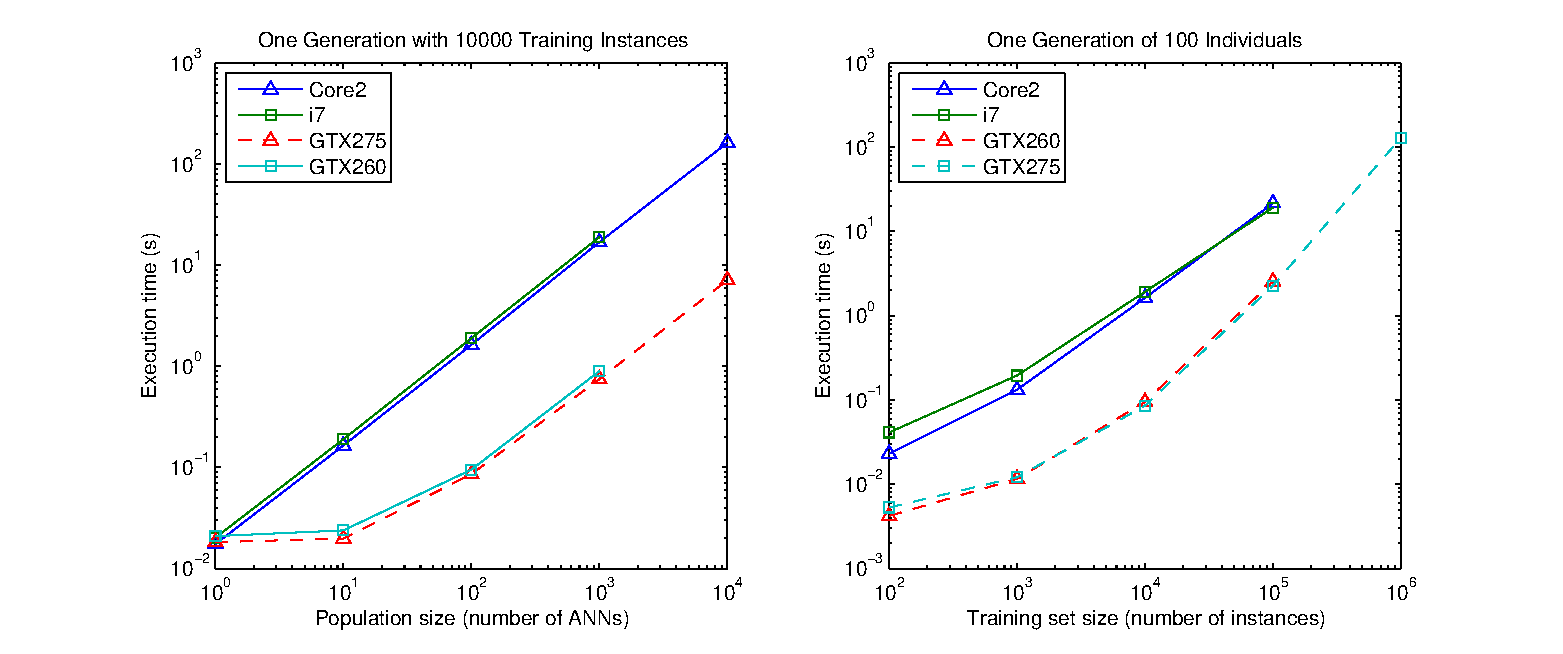
\includegraphics[width=\textwidth]{fig-performance}
	\caption{Training performance as a function of population size (left) and training set size (right). Note logarithmic axes.}
	\label{fig:training-performance}
\end{figure}

% ----------------------------------------------------------------------------
\subsection{Classifier Results} \label{results}
% ----------------------------------------------------------------------------

% ############################################################################
\section{Conclusion} \label{concl}
% ############################################################################
We have presented an implementation of GA training of ANN classifiers for the CUDA platform for GPU programming. By carefully designing memory organization, algorithm computational load and memory access patterns, we have obtained a 10-fold speedup compared to a conventional sequential CPU implementation. Additional workaround were necessary for the low amount of fast on-chip GPU memory. Our method scales across population and training set sizes.

% ############################################################################
\section{Discussion} \label{disc}
% ############################################################################

% ----------------------------------------------------------------------------
\subsection{Future Work} \label{future}
% ----------------------------------------------------------------------------
Montana and Lawrence \cite{GA-ANN} have demonstrated that a brief period of hill climbing after training with a genetic algorithm may increase the accuracy of classifier results. Thus, we could improve the accuracy of our methods by incorporating hill-climbing methods, such as the parallel backpropagation method described by Oei, Friedland and Janin \cite{backprop}.


% ############################################################################
% Bibliography
% ############################################################################
\bibliographystyle{plain}
\bibliography{bibliography}     %loads bibliography.bib

% ============================================================================
\end{document}
% ============================================================================
